\subsection{IFIT2A}
\subsubsection{Human and Monkey IFIT2 in a Simplified System of pseudo-IBs} \label{Human and Monkey IFIT2 in a Simplified System of pseudo-IBs}
\myparagraph{Nascent Human and Monkey IFIT2 in pIBs}
\mysubparagraph{i2a 293t hnhp}
Cell Line: 293T \newline
Treatment: hNhP \newline
Detecting magenta: endogenous human IFIT2 \newline
Detecting cyan: human pIB \newline

Nascent human IFIT2 strongly concentrates within the human RSV pseudo inclusion bodies.

\begin{figure}
    \centering
    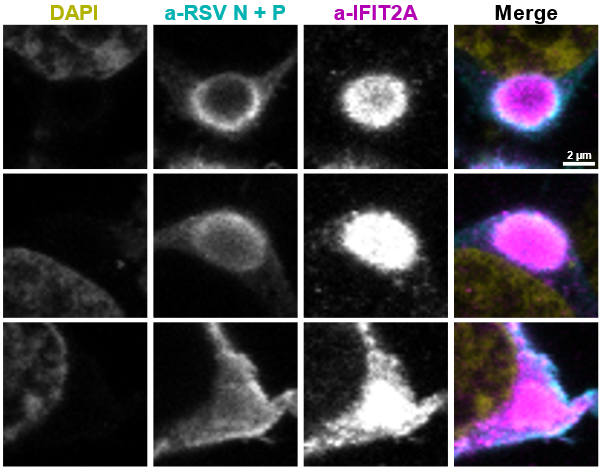
\includegraphics[width=1\linewidth]{09. Chapter 4//Figs//01. I2A/01. i2a 293t hnhp.png}
    \caption[i2a 293t hnhp]{i2a 293t hnhp}
    \label{i2a 293t hnhp}
\end{figure}

\mysubparagraph{i2a vero hnhp}
Cell Line: VERO \newline
Treatment: hNhP \newline
Detecting magenta: endogenous monkey IFIT2 \newline
Detecting cyan: human pIB \newline

Endogenous monkey IFIT2 colocalises with the pIB structure (probably like an inclusion), as well as with the pIB filamentous network.

\begin{figure}
    \centering
    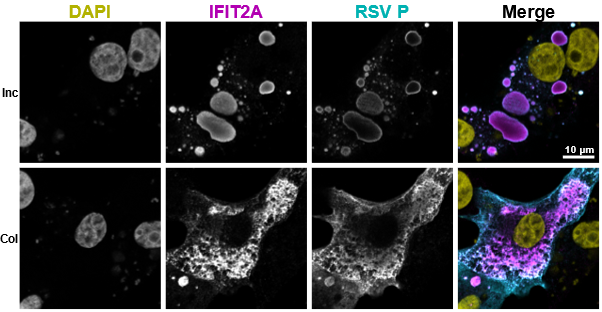
\includegraphics[width=1\linewidth]{09. Chapter 4//Figs//01. I2A/02. i2a vero hnhp.png}
    \caption[i2a vero hnhp]{i2a vero hnhp}
    \label{i2a vero hnhp}
\end{figure}

\myparagraph{Exogenous Human and Bovine IFIT2 in pBs}
\mysubparagraph{i2a vero hi2 + hnhp}
Cell Line: VERO \newline
Treatment: hNhP + hIFIT2-FLAG \newline
Detecting magenta: endogenous monkey IFIT2 + exogenous human IFIT2 \newline
Detecting cyan: human pIB \newline

Monkey cells transfected with human RSV N and P, along with human IFIT2-FLAG show concentration within the pIB structures as well as the pIB filamentous network. In this experiment we are detecting both human and monkey IFIT2, however we can see a huge difference in IFIT2 expression between some cells (bottom panel; cells in the periphery of the picture), suggesting that what we are mainly detecting is the overexpressed human IFIT2-FLAG.

\begin{figure}
    \centering
    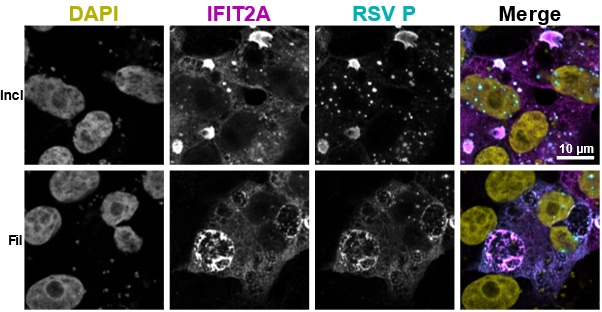
\includegraphics[width=1\linewidth]{09. Chapter 4//Figs//01. I2A/03. i2a vero hi2 hnhp.png}
    \caption[i2a vero hi2 + hnhp]{i2a vero hi2 + hnhp}
    \label{i2a vero hi2 + hnhp}
\end{figure}

\subsubsection{Nascent Human and Bovine IFIT2A Localisation During h/bRSV Infection} \label{Nascent Human and Bovine IFIT2A Localisation During h/bRSV Infection}
\myparagraph{hIFIT2A localisation during hRSV Infection}
\mysubparagraph{i2a a549 hrsv}
Cell Line: A549 \newline
Treatment: hRSV \newline
Detecting magenta: endogenous human IFIT2  \newline
Detecting cyan: human IB \newline

Nascent human IFIT2 shows 3 phenotypes with regards to colocalization with human RSV N. It seems to colocalise to the edge of the IB structure, with a partial signal also being detected in the inner edge of the structure (top panel); it completely colocalises to the N staining (middle panel; could be because the section is going through the top of the IB sphere); or forms inclusion inside the IB structure (bottom panel. 

\begin{figure}
    \centering
    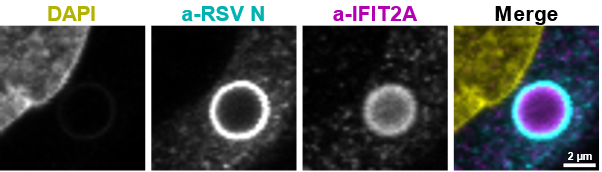
\includegraphics[width=1\linewidth]{09. Chapter 4//Figs//01. I2A/04. i2a a549 hrsv n.png}
    \caption[i2a a549 hrsv n]{i2a a549 hrsv n}
    \label{i2a a549 hrsv n}
\end{figure}

Cell Line: A549 \newline
Treatment: hRSV \newline
Detecting magenta: endogenous human IFIT2  \newline
Detecting cyan: human IB \newline

Nascent human IFIT2 colocalises with the ring structure (outlined by RSV P staining) and to the inner edge of the IB.

\begin{figure}
    \centering
    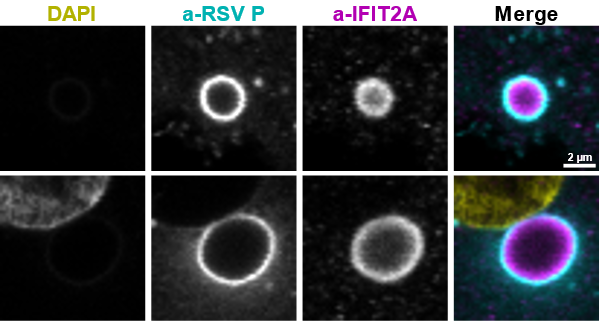
\includegraphics[width=1\linewidth]{09. Chapter 4//Figs//01. I2A/05. i2a a549 hrsv p.png}
    \caption[i2a a549 hrsv p]{i2a a549 hrsv p}
    \label{i2a a549 hrsv p}
\end{figure}

Cell Line: A549 \newline
Treatment: hRSV \newline
Detecting magenta: endogenous human IFIT2  \newline
Detecting cyan: human IB \newline

With regards of colocalization with human RSV M2/1 protein, human IFIT2 seems to either form inclusion, which has a signal decrease towards the middle of the IB structure (top panel), or seems to strongly colocalise with the ring structure highlighted by M2/1 staining (bottom 2 panels; there also seems to be IFIT2 signal concentration on the inner edge of the IB structure).

\begin{figure}
    \centering
    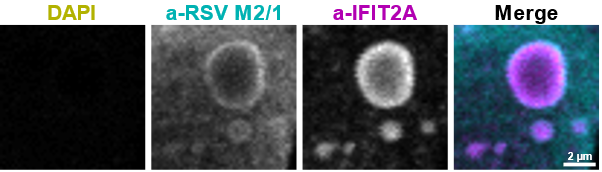
\includegraphics[width=1\linewidth]{09. Chapter 4//Figs//01. I2A/06. i2a a549 hrsv m21.png}
    \caption[i2a a549 hrsv m21]{i2a a549 hrsv m21}
    \label{i2a a549 hrsv m21}
\end{figure}

\mysubparagraph{i2a beas2b hrsv}
Cell Line: BEAS2B \newline
Treatment: hRSV \newline
Detecting magenta: endogenous human IFIT2  \newline
Detecting cyan: human IB \newline

\begin{figure}
    \centering
    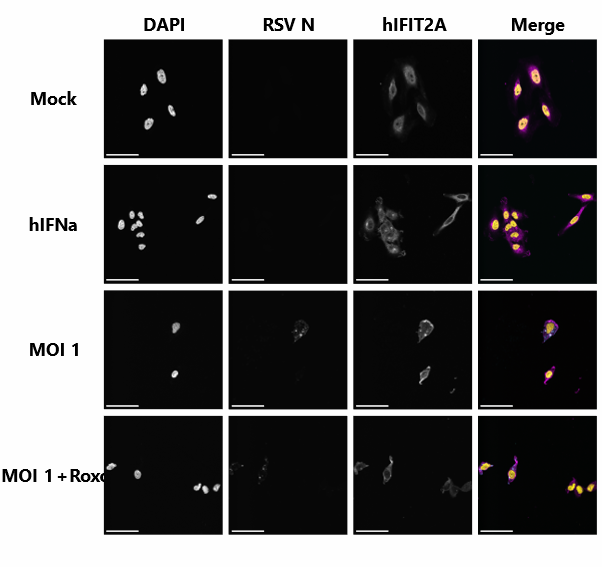
\includegraphics[width=1\linewidth]{09. Chapter 4//Figs//01. I2A/07. i2a beas2b hrsv.png}
    \caption[i2a beas2b hrsv]{i2a beas2b hrsv}
    \label{i2a beas2b hrsv}
\end{figure}

\myparagraph{hIFIT2A localisation during bRSV Infection}
\mysubparagraph{i2a mdbk brsv}
Cell Line: MDBK \newline
Treatment: bRSV + bIFNa \newline
Detecting magenta: endogenous bovine IFIT2  \newline
Detecting cyan: bovine IB \newline

Nascent bovine IFIT2 colocalization with regards of N stained bRSV IBs seems to strongly associate with the ring of the structure.

\begin{figure}
    \centering
    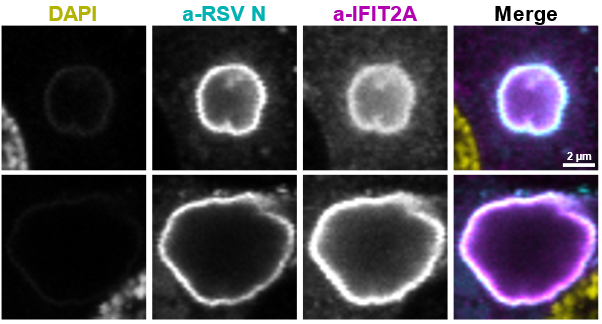
\includegraphics[width=1\linewidth]{09. Chapter 4//Figs//01. I2A/08. i2a mdbk brsv.png}
    \caption[i2a mdbk brsv]{i2a mdbk brsv}
    \label{i2a mdbk brsv}
\end{figure}

\subsection{Summary} \label{Summary-i2a}
Both endogenous human and monkey IFIT2 forms inclusions inside human RSV pseudo-IBs. Monkey IFIT2 also colocalises to the pIB filamentous network (this structure was not observed in the human experiment). The identical staining can be observed in monkey cells with overexpressed human IFIT2-FLAG. Nascent human IFIT2 during hRSV infection consistently localises to the IB structure. It seems to have preference for the ring and the inner edge of the structure; however, we have seen it as homogenous inclusion as well. Endogenous bovine IFIT2 colocalises to the ring of the IB during bRSV infection.